%%!TEX root = diss.tex

\chapter{From particle dynamics to the sediment flux}
\label{ch:flux}
\section{Introduction}

A relativity weak flow shearing a bed of sediment entrains individual particles into a state of motion controlled by turbulent forcing and intermittent collisions with other grains at rest on the bed, generating wide fluctuations in the sediment velocity \citep{Heyman2016,Fathel2015}.
Bedload particles move downstream until they are disentrained when they happen to encounter sufficiently sheltered pockets on the bed surface to interrupt their motions \citep{Charru2004,Gordon1972}.
Eventually, the bed around them rearranges and destroys this shelter, or turbulent fluctuations overcome the shelter \citep{Celik2014,Valyrakis2010}, and particles are once again entrained.
Bedload transport is thus a kind of intermittent motion, characterized by alternation between fluctuating movements and periods of rest.

To date, descriptions of bedload transport have therefore simplified the problem in various ways to enable progress.
The foundational work is due to Einstein, who considered bedload motions as instantaneous so he could describe bedload transport as an alternating sequence of ``steps" and rests having random length and duration \citep{Einstein1937}, in a pioneering application of the continuous time random walk \citep{Montroll1965}.
Einstein concluded that particles move downstream with a mean velocity $\bra u \ket = k_E \ell$, where $k_E$ is the rate at which the individual bed particle is entrained into motion, and $\ell$ is the mean length of each downstream step.
Later, Einstein applied these ideas to calculate the mean downstream flux due to the movements of many such particles \citep{Einstein1950}. Einstein reasoned that if the density of resting particles on the bed is $\rho_b$, the overall areal entrainment rate of particles can be written $E = \rho_b k_E$, giving a mean sediment flux $\bra q \ket = \rho_b \bra u \ket  = E \ell $.

Many researchers have since refined Einstein's approach to provide more realistic descriptions of individual particle motions than his instantaneous step model.
One set of efforts has neglected the particle deposition process to calculate the downstream velocity distributions of moving particles using mechanistic equations with noise terms representing turbulent fluid forces and particle-bed collisions \citep{Ancey2014,Fan2014}. 
Another set of works have described particles alternating between motion and rest considering that motions occur with a constant velocity \citep{Lisle1998,Lajeunesse2017}. 
No models have yet been formulated which describes particles alternating between motion and rest with motions having realistic fluctuating velocities, even though this is how bedload particles actually move.
A more realistic description of particle velocities during individual movements has potential to improve our understanding of bedform initation and particle-particle interactions in subsequent developments.

Parallel to these efforts to better describe individual particle trajectories, a complementary set of studies produced stochastic formulations of the sediment flux which improve on the mean field description provided by Einstein \citep{Turowski2010,Furbish2012a,Ancey2020}. 
Sediment fluxes generally exhibit wide fluctuations due to variations in the number of moving particles and their velocities \citep{Bohm2005a,Ancey2006,Furbish2012a}, the migration of bedforms and sediment waves \citep{Guala2014,Recking2012}, and a host of other processes \citep{Dhont2018}.
Because these fluctuations occur over disparate timescales, measurements of mean sediment fluxes depend on the timescale over which they are collected, a phenomenon called scale dependence \citep{Saletti2015,Dhont2018,Singh2009,Turowski2010,Ancey2020}.
To date, very few models have calculated the probability distribution of the bedload sediment flux due to individual particle motions \citep{Ancey2008,Ancey2014}, and among these, even fewer have described any observation-scale dependence of the flux \citep{Ancey2020a,Turowski2010}.
Among those that do include scale dependence, none formulate the sediment flux in terms of the trajectories of individual grains.

This survey provides context for the two problems addressed in this chapter.
First, we lack the capability to describe individual sediment trajectories through motion and rest including velocity fluctuations in the motion state; and second, we need more understanding of how to connect individual particle trajectories through motion and rest to the overall streamwise sediment flux, including its probability distribution and the dependence of its statistical moments on the observation time.

Here, I develop a new statistical physics-based formalism which addresses both of these problems by describing individual particle trajectories with a stochastic Langevin equation.
This dynamical equation describes alternation between motion and rest at random intervals while particles in motion have velocity that fluctuates around a mean value.
Using the probability distribution of particle position generated by this model, I construct a formalism to derive analytically the probability distribution of the sediment flux.
This distribution exhibits observation-scale dependence as a result of velocity fluctuations among moving particles.
Below, I develop the new formalism in Sec. \ref{sec:mod}, solve it in Sec. \ref{sec:res}, and discuss the implications of my results and future research ideas in Secs. \ref{sec:disc} and \ref{sec:conc}.

\section{Description of motion-rest alternation with velocity fluctuations \label{sec:mod}}
The starting point for this analysis is an idealized one-dimensional domain, infinite in extent, populated with sediment particles on the surface of a sedimentary bed.
Particles are set in motion by the turbulent flow and move downstream until they deposit, and the cycle repeats.
The downstream coordinate is $x$, so that $\dot{x}$ describes a velocity in the downstream direction.
The flow is considered weak enough that interactions among moving grains are very rare, although interactions between moving particles and the bed may be common, characteristic of rarefied transport conditions \citep[e.g.][]{Kumaran2006,Furbish2017}. 
Particles are considered to have similar enough shapes and sizes so as to have nearly identical mobility characteristics.
These conditions allow for all particles to be described as independent from one another but governed by the same underlying dynamical equations.

\subsection{Dynamical equation for grain-scale sediment transport}
From these assumptions, the first target is to write an equation of motion for the individual sediment particle encompassing two features.
\begin{figure}
	\centerline{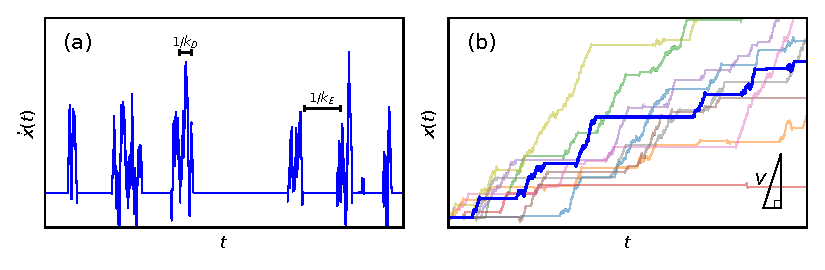
\includegraphics{./figures/ch2/fig0mod.pdf}}
	\caption{Panel (a) sketches a realization of the noise in equation \ref{eq:flippylangevin}, while panel (b) shows the trajectory derived from it (in blue) alongside other possible trajectories. Keys in panel (a) demonstrate the average movement time $1/k_D$ and rest time $1/k_E$, while the key in panel (b) shows the average movement velocity $V$. Velocity fluctuations produce tilted stair-step trajectories with unsteady slopes in the $x-t$ plane. This can be compared with Fig. \ref{fig:lislefig} which does not include fluctuations.}
	\label{fig:fluxxy0}
\end{figure}
First, particles should alternate between motion and rest.
The entrainment transition rate from rest to motion occurs with probability per unit time (or rate) $k_E$, while the deposition transition from motion to rest occurs with rate $k_D$.
Second, particles in motion should move with mean velocity $V$ as their instantaneous velocities jitter around this mean value due to turbulent drag and particle-bed collisions.

The simplest equation of motion including these features is
\be \dot{x}(t) = [V + \sqrt{2D}\xi(t)]\eta(t).  \label{eq:flippylangevin} \ee
Here,  $\xi(t)$ is a Gaussian white noise having zero mean and unit variance representing velocity fluctuations among moving particles. $\eta(t)$ is a dichotomous noise which takes on values $\eta = 1$, representing motion (with mean duration $1/k_D$), and $\eta=0$, representing rest (with mean duration $1/k_E$).
The transition rate from $\eta=0$ to $\eta = 1$ is $k_E$, and the transition rate from $\eta=1$ to $\eta= 0$ is $k_D$. The notation $k=k_E+k_D$ is a shorthand used throughout the thesis.
Times spent in motion and rest are respectively distributed as $P(t) = k_D \exp(k_D t)$ and $P(t) = k_E \exp(k_E t)$.
$V$ is the mean particle velocity describing the overall downstream drift of moving particles, while $D$ is a diffusivity [units $L^2/T^3$] describing velocity fluctuations among moving particles.



Equation \ref{eq:flippylangevin} describes the downstream movement of particles alternating through motion and rest with velocity fluctuations in the motion state.
This model can be understood as a generalization of the ``randomly flashing diffusion" models developed by Luczka and coworkers in physics \citep{Luczka1992,Luczka1993,Luczka1995}.
Some trajectories produced by the Langevin equation \ref{eq:flippylangevin} are sketched in Fig. \ref{fig:fluxxy0}.
The driving term in panel (a) displays excessive fluctuations due to the assumption that velocities evolve as Gaussian white noise with no temporal correlations, but the integrated particle trajectories in panel (b) are well-behaved and visually similar to those of earlier studies \citep[cf.][]{Fan2016,Bialik2015}.

Eq. \ref{eq:flippylangevin} generalizes the constant velocity model of \citet{Lisle1998} and \citet{Lajeunesse2017} that was presented in section \ref{sec:lisle}, providing the first extension of these works aimed at a refined description of bedload particle trajectories through motion and rest.


\subsection{Derivation of the master equation for the sediment position distribution}
\label{sec:floppymastereq}
The solution of equation \ref{eq:flippylangevin} for a given realization of the two noises $\eta(t)$ and $\xi(t)$ gives one possible trajectory of a particle. The probability distribution $P(x,t)$ that a particle which started at position $x=0$ at time $t=0$ has traveled to position $x$ by time $t$ can be formulated as an average over the ensemble of all possible trajectories.

This probability distribution of position is formed as $ P(x',t) = \big\bra \delta(x'-x(t))\big\ket_{\eta,\xi} $, where $x(t)$ is the formal solution of Eq. \ref{eq:flippylangevin} and the average is over both noises.
This symbolic equation is not directly useful as taking averages over both noises is a challenging mathematical problem \citep[e.g.][]{Hanggi1978}. This calculation is completed in the appendix Sec. \ref{sec:appAmaster}, providing the master equation
\be (\pt^2 + V \px \pt + k_E V \px + k \pt - D \px^2 \pt - k_E D \px^2) P(x,t) = 0 \label{eq:flippymaster}\ee
for the position probability distribution.
The master equation \ref{eq:flippymaster} is a diffusion-like equation governing the probability distribution of position for individual particles alternating between motion and rest, with the movement velocity considered as a fluctuating quantity.

One can see in particular that taking the entrainment rate $k_E$ very large, meaning that particles are very often moving, implies a classical advection-diffusion equation $(\pt + V\px -D \px^2)P=0$ for the position, characteristic of a particle moving downstream with Gaussian velocity fluctuations. Otherwise, there is a possibility that the particle is at rest and the advection-diffusion process is interrupted, giving rise to the additional terms in Eq. \ref{eq:flippymaster} and providing an asymmetrical structure reminiscent of Eq. \ref{eq:lislemaster} from the simpler motion-rest models of Sec. \ref{sec:lisle}.

\section{Formalism for the downstream sediment flux}
\label{sec:flippyflux}

The probability distribution of the sediment flux can be calculated using the probability distribution of particle position $P(x,t)$ derived as the solution of Eq. \ref{eq:flippymaster}.
This method is modified from the approach recently developed by Banerjee and coworkers in physics \citep{Banerjee2020}.
This generalizes the nonlocal formulation of Sec. \ref{sec:nonlocal} to provide the probability distribution of the flux, and it re-frames the renewal approach of Sec. \ref{sec:renewal} in terms of the mechanics of individual particles in transport.

The basic idea, as depicted in Fig. \ref{fig:flipflopfig1}, is to initially distribute $N$ particles in all states of motion along a domain of length $L$ at some random initial locations $x_i$ to the left of $x=0$.
Later, the number of particles $N$ and the size $L$ of the domain will be extended to infinity such that their ratio $\rho=N/L$ remains constant. 
This limit will provide a configuration similar to the one constructed in the nonlocal formation (Sec. \ref{sec:nonlocal}).

From this initial configuration, particles move downstream through time according to Eq. \ref{eq:flippylangevin}.
The flux is calculated as the average rate of particles crossing to the right of the control surface (at $x=0$) after the sampling time $T$.
\begin{figure}
	\centerline{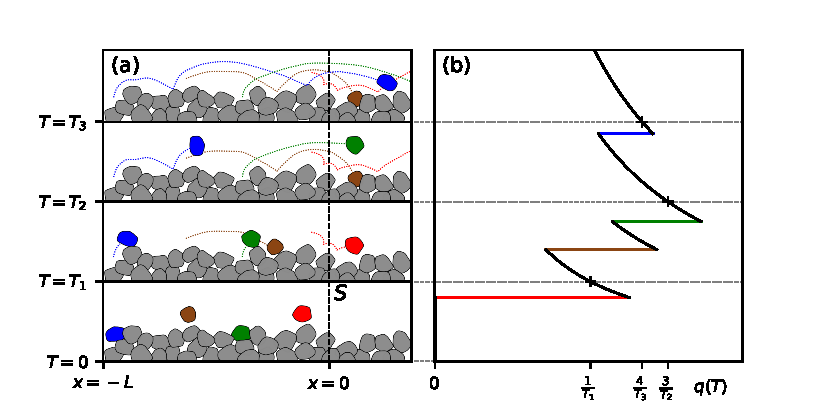
\includegraphics{./figures/ch2/figure1.pdf}}
	\caption{The left panel indicates the configuration for the flux. The particle trajectories within demonstrate alternation between rest and motion with fluctuating velocity. Particles begin their transport with positions $-L\leq x \leq 0$ at $t=0$, and as depicted in the right panel, the flux is calculated with the number of particles $N_>(T)$ which lie to the right of $x=0$ at the observation time $t=T$, divided by $T$: $q(T) = N_>(T)/T$. The probability distribution of $q(T)$ is determined from all possible realizations of the trajectories and initial positions as $N,L$ tend to infinity while the density of particles $\rho=N/L$ to the left of the control surface remains fixed.}
	\label{fig:flipflopfig1}
\end{figure}
This time-averaged flux is
\be q(T) = \frac{1}{T}\sum_{i=1}^N I_i(T). \label{eq:flippyflux} \ee
In this equation, the $I_i(T)$ are indicator functions which equal $1$ if the $i$th particle has passed the control surface ($x=0$) at the observation time $T$ and $0$ otherwise.
All particles which have not crossed the control surface (or which have crossed and then crossed back) do not contribute to the flux.

The probability distribution of the flux is then the average of Eq. \ref{eq:flippyflux} across all possible initial configurations of particles and their trajectories
\be P(q|T) = \Big \bra \delta\Big( q - \frac{1}{T}\sum_{i=1}^N I_i(T) \Big) \Big\ket. \ee
These averages are again most easily conducted in Laplace space. 
Taking the Laplace transform over $q$ (i.e. forming the characteristic function of $P(q|T)$) obtains
\begin{align} \tilde{P}(s|T) &=  \Big\bra \exp\Big(\frac{s}{T}\sum_{i=1}^N I_i(T)\Big)\Big\ket \\
	&=  \prod_{i=1}^N \Big\bra \exp\Big(-\frac{s}{T}I_i(T)\Big)\Big\ket \\
	&= \prod_{i=1}^N \Big[1-\big(1-e^{-s/T}\big)\big\bra I_i(T) \big\ket \Big] \label{eq:flippycharacteristic}\end{align}
This progression relies on the independence of averages for each particle (so the average of a product is the product of averages) and the observation that  $e^{a I} = 1-(1-e^a)I$ because $I$ is either $0$ or $1$.

The average over initial conditions and possible trajectories for the $i$th particle involved in this characteristic function can be written
\be \bra I_i(t) \ket = \frac{1}{L}\int_{-L}^0 dx' \int_0^\infty dx P(x-x',t) \label{eq:indicator} \ee
where $P(x,t)$ is the position probability distribution which solves Eq. \ref{eq:flippymaster}.
Eq. \ref{eq:indicator} describes the probability that the $ith$ particle is found to the right of control surface by time $T$ provided it started at a random location somewhere to the left.
These $\bra I_i(t) \ket$ are the components of the flux that depend on the particle dynamics. 

Inserting Eq. \ref{eq:indicator} into Eq. \ref{eq:flippycharacteristic} and taking the limits $L\rightarrow \infty$ and $N \rightarrow \infty$ as the density of particles $\rho = N/L$ remains constant, producing the configuration of the nonlocal formulation in section \ref{sec:nonlocal}, provides
\begin{align} \tilde{P}(s|T) &= \lim_{N \rightarrow \infty} \Big(1 - \frac{1}{N}\big(1-e^{-s/T}\big)\Lambda(T) \Big)^N \\ &= \exp \Big[ -\big(1-e^{-s/T}\big)\Lambda(T) \Big]. \label{eq:flippychar} \end{align}
where $\Lambda(T) = \rho \int_0^\infty dx \int_0^\infty dx' P(x+x',T)$ is a rate \textit{function}, similar to the rate constant in the renewal process models of section \ref{sec:renewal}, except that it is now formulated in terms of individual particle trajectories via the probability distribution of particle position $P(x,t)$, which itself originates from the Langevin equation \ref{eq:flippylangevin} governing the particle dynamics.

Eq. \ref{eq:flippychar} is the characteristic function of a Poisson distribution \citep{Cox1965}.
Expanding in $e^{-s/T}$ and inverting the Laplace transform provides a key equation of this chapter, the probability distribution of the flux held contingent on the sampling time $T$:
\be P(q|T) = \sum_{l=0}^\infty \frac{\Lambda(T)^l}{l!}e^{-\Lambda(T)}\delta(q-\frac{l}{T}). \label{eq:flippydist}\ee
This equation implies that the mean flux is $\bra q(T) \ket = \int_0^\infty q P(q|T) dq = \Lambda(T)/T$. Similarly the variance is $\sigma_q^2(T) = \Lambda(T)/T^2$. For the case when $\Lambda(T)$ is proportional to the observation time ($\Lambda \propto T$), these formulas become identical to the renewal theory approach reviewed in section \ref{sec:renewal}.
This correspondence demonstrates that the renewal approach can be formulated equivalently by considering the dynamics of individual particles as a starting point.

\section{Results \label{sec:res}}
\subsection{Position probability distribution of sediment particles}
\begin{figure}
	\centerline{\includegraphics{figures/ch2/figure2_slopeKey.pdf}}
	\caption{Panel (a) indicates the probability distribution of particle position (Eq. \ref{eq:monster}) as it evolves through time. From the initial mixture of motion and rest states, particles advect downstream as they diffuse apart from one another due to differences in their velocities and transition times between motion and rest. In panel (a), the initial position persists as a Delta-function spike for the black $t=10\tau$ curve. Panel (b) shows the resulting particle diffusion (Eq. \ref{eq:diffo}). At timescales $t \ll 2D/V^2$, the diffusion is normal since the movement is approximately a standard Brownian diffusion process. For larger timescales, $2D/V^2 \ll t \ll \tau$, particles undergo ballistic diffusion similar to \citet{Lisle1998} as a result of some particles being stationary as others advect. Finally at times longer than the timescale $\tau = 1/k$ associated with entrainment and deposition, diffusion is again normal, formed of particles well-mixed among motion and rest states. All results are scaled by the mean hop length $\ell=V/k_D$ and the timescale $\tau=1/k$ of the motion/rest alternation. In both plots, the lines are analytical results while the points are the results of Monte Carlo simulations based on evaluating cumulative transition probabilities on a small time-step \citep[e.g.][]{Barik2006}.}
	\label{fig:flippyfig1}
\end{figure}
The master equation \ref{eq:flippymaster} describes the evolution of the probability distribution of position through time. The solution of this equation should be some combination of the \citet{Einstein1937} theory for particle transport (section \ref{sec:einwalk}) with the Gaussian solution of the advection-diffusion equation \citep[e.g.][]{Morse1953}.

Because the master equation is second order in time, it requires initial conditions for both $P$ and $\pt P$. Considering that particles start at rest in a mixture of motion and rest states, with a fraction $k_E/k$ starting in motion and a fraction $k_D/k$ starting in rest, these conditions derive from the initial state 
\be P(x,0) = \lim_{t\rightarrow 0 } \frac{k_E}{k} \sqrt{\frac{1}{4\pi D t}} \exp\Big[-\frac{(x-Vt)^2}{4Dt}\Big]+ \frac{k_D}{k}\delta(x)\ee
which gives $P(x,0) = \delta(x)$ and $ \pt P(x,0) = \frac{k_E}{k}\big[D\delta''(x)-V \delta'(x) \big]$ \citep[cf.][]{Weiss2002a}.

The master equation \ref{eq:flippymaster} is solved by transform calculus in section \ref{sec:fluccymastersol} of the appendix, providing
\begin{multline} P(x,t) = \big[-\varphi D\px^2 + V\varphi \px + k + \delta(t) +  \pt \big]\\
	\times \int_0^t \mathcal{I}_0\Big( 2 \sqrt{k_Ek_D u(t-u)}\Big) e^{-k_E(t-u)-k_D u} \\ \times \sqrt{ \frac{1}{4\pi D u}} \exp\Big[- \frac{(x-Vu)^2}{4Du}\Big] du, \label{eq:monster}
 \end{multline}
where $\varphi=k_D/k$ is the probability the particle starts at rest and $\mathcal{I}_0$ is a modified Bessel function. This equation generalizes the earlier result  \ref{eq:lisledist} for alternation between motions and rests to include velocity fluctuations within the motion state.

The distribution Eq. \ref{eq:monster} is shown evolving through time in Fig. \ref{fig:flippyfig1} panel (a), where the advection and diffusion characteristics of Eq. \ref{eq:flippymaster} are both evident. The integral in Eq. \ref{eq:monster} encodes the earlier expectation of Einstein model-like behavior mixed with a Gaussian propagator, in that it convolves the Bessel function probability that the particle has been in motion for a period $u$ out of a time $t$ with the Gaussian probability that a particle has traveled a distance $x$ in time $u$ within the motion state. The prefactors of this integral term can be understood as adapting this distribution to the initial conditions.

\subsection{The moments of particle position through motion-rest alternation}

The moments of position produced by Eq. \ref{eq:monster} could be derived by integrating it directly, but this is difficult. Instead, the moments can be calculated directly from the master equation \ref{eq:flippymaster} \citep[e.g.][]{Cox1965}. 

Multiplying Eq. \ref{eq:flippymaster} by $x^l$ and integrating over all $x$ provides
\begin{multline} \pt^2 \bra x^l \ket -V l \pt \bra x^{l-1} \ket -k_E V l \bra x^{l-1} \ket + k \pt \bra x^{l} \ket\\- D l (l-1) \pt \bra x^{l-2} \ket - k_E D l(l-1) \bra x^{l-2} \ket = 0.\end{multline}
For $l = 1$, this equation generates the mean position $ \bra x \ket(t) = k_E V t/k$, which is unaffected by diffusion (since Gaussian velocity fluctuations are symmetric).
The case $l=2$ provides the second moment, implying the variance of position is
\be \sigma_x(t)^2 = \frac{2k_Ek_DV^2}{k^3}\Big( t + \frac{1}{k}e^{-k t} - \frac{1}{k}\Big) + 2\frac{k_E D}{k}t. \label{eq:minor} \ee
This equation describes a non-trivial multi-scale diffusion phenomenon, whereby the rate at which particles spread apart from one another depends on how long their dynamics have been ongoing.


Provided that $2D/V^2 \ll k_D/k^2$, series expansion of \ref{eq:minor} in $t$ and $1/t$ reveals three different scaling behaviors:
\be \sigma_x^2 \sim 
\begin{cases}
	 t, & t \ll \frac{2Dk}{V^2 k_D}, \\ 
	 t^2, &  \frac{2Dk}{V^2 k_D} \ll t \ll \frac{1}{k}, \\
	 t, & t\gg \frac{1}{k}. \label{eq:diffo}
\end{cases} \ee
Note in the physical condition when $k\approx k_D$, which is generally satisfied for bedload transport since motions are typically short compared to rests \citep{Hassan1991,Wu2019}, the above condition for existence of three ranges becomes $ \Pe \gg 1,$ where
$\Pe =V^2/(2k_D D)$ is a P\'{e}clet number \citep[e.g.][]{Heyman2014}. This P\'{e}clet number measures the relative importance of advection and diffusion to the downstream movements of particles.

The large P\'{e}clet limit ($\Pe\gg 1$) is the physically-relevant condition for bedload transport, where velocity fluctuations are typically small compared to mean downstream movement velocities, so that particles rarely move upstream any appreciable distance \citep[e.g.][]{Fathel2015}. This limit also generates the three-range diffusion exemplified by Eq. \ref{eq:diffo}, so we should expect bedload particles to spread apart with three different scaling ranges depending on how long they have been observed \citep[cf.][]{Nikora2001,Nikora2002}, at least within the assumptions of the model.
Fig. \ref{fig:flippyfig1} panel (b) sketches the predicted three-range diffusion, which is discussed further in Sec. \ref{sec:prollems}.

Below, this anomalous diffusion behavior \citep[cf.][]{Sokolov2012} is shown to affect the rate constant $\Lambda(t)$ in the sediment flux. As a result of these multi-scale particle dynamics, the sediment flux becomes scale-dependent in a richer way than the renewal model of section \ref{sec:renewal}.

\subsection{Calculation of the sediment flux}

From the formalism in Sec. \ref{sec:flippyflux}, the central parameter of the sediment flux distribution is the rate function
\be \Lambda(t) = \rho \int_0^\infty dx_i \int_0^\infty dx P(x+x_i,t). \label{eq:flatform}\ee
This represents the number of particles crossing $x=0$ at the observation time $T$ given they started somewhere to left of $x=0$ at $T=0$.

Using the probability distribution of position Eq. \ref{eq:monster}, the integrals in Eq. \ref{eq:flatform} are performed in appendix Sec. \ref{sec:fluxconstant}u, providing the rate function
\begin{multline} 
\Lambda(t) = \rho \int_0^t \mathcal{I}_0\Big(2\sqrt{k_Ek_Du(t-u)}\Big)e^{-k_E(t-u)-k_D u} \\
\times \Bigg[\sqrt{\frac{D}{\pi u}}\Big([\cev{\partial_t} + k]u-\frac{k_D}{2 k}\Big)e^{-V^2 u/4D} \\+ \frac{V}{2}\Big([\cev{\partial_t} + k]u -\frac{k_D}{k}\Big) \erfc\Bigg(-\sqrt{\frac{V^2 u}{4D}}\Bigg)\Bigg] du. \label{eq:fluxy}
\end{multline}
In this equation, the notation $\cev{\partial_t}$ means that the partial time derivative acts from the left of all terms in which it is involved, as in $f(t)\cev{\partial_t} g(t) = \partial_t [f(t)g(t)].$

This is an intricate result for the rate function in the sediment flux distribution Eq. \ref{eq:flippydist}. This mathematical complexity may not be surprising given that Eq. \ref{eq:flippylangevin} involves two interacting diffusion processes. As displayed in Fig. \ref{fig:fluxconvergence}, as a result of Eq. \ref{eq:fluxy} the mean sediment flux takes on a non-trivial scale-dependence, characterized by a decay toward the Einstein prediction $q_0 = \rho k_E V/k = E \ell$ as the observation time becomes much larger than $1/(k_D \Pe)$. 
\begin{figure}[!htbp]
	\includegraphics[width=\linewidth,keepaspectratio]{figures/ch2/figure3_slopeKey.pdf}
	\caption{The mean sediment flux is plotted for different values of the P\'{e}clet number $\Pe = V^2/(2k_D D)$, characterizing the relative strength of particle velocity fluctuations during motion. The flux is normalized by the prediction $q_0 = E \ell$ of the Einstein theory (Sec. \ref{sec:einflux}). For nonzero velocity fluctuations in the motion state (finite $\Pe$), the Einstein limit is approached as the observation time $T$ grows. Stronger velocity fluctuations (smaller $\Pe$) slow the convergence to this limit.
	In all cases, satisfactory convergence of the mean flux is achieved when the observation time satisfies $T\gg 1/(k_D \Pe),$ as expected by Eq. \ref{eq:fluccolimitcases}. Plotted lines are the analytical result Eq. \ref{eq:fluxy}, while the points are the results of Monte Carlo simulations. Vertical dotted lines indicate the convergence time $T = (k_D \Pe)^{-1}$ for each condition. }
	\label{fig:fluxconvergence}
\end{figure}

Further insight into the rate constant of the sediment flux distribution can be gained by investigating extreme cases of the observation time.
As shown in appendix Sec. \ref{sec:fluxlimits}, Eq. \ref{eq:fluxy} takes on relatively simple forms at extreme values of $T$: 
\be \Lambda(T) =
\begin{cases}
 \frac{\rho k_E}{k}\sqrt{\frac{D T}{\pi}}	& T \ll (k_D \Pe)^{-1} \\
 \frac{\rho k_E V T}{k} & T \gg (k_D \Pe)^{-1}. 
\end{cases}
\label{eq:fluccolimitcases}
\ee

Since the mean flux is $\bra q(T) \ket = \Lambda(T)/T$, the condition on the observation time so that the flux converges to the Einstein value $q_0 = \rho k_E V/k = E \ell$ can be expressed as $T\gg (k_D \Pe)^{-1}$. It is related to the P\'{e}clet number and is proportional to the time particles spend in motion ($1/k_D$). As a result, when particle velocity fluctuations during motions become large comparable to the mean particle velocity, Eq. \ref{eq:fluccolimitcases} indicates that the flux becomes slow to converge to the Einstein result.

\section{Discussion \label{sec:disc}}

This chapter has generalized the earlier descriptions of individual sediment trajectories \citep[e.g.][]{Lisle1998,Lajeunesse2017} to include velocity fluctuations in the motion state.

Using results from this generalized model as an example, I demonstrated how to calculate the sediment flux probability distribution, phrasing earlier renewal theory approaches (Sec. \ref{sec:renewal}) more directly in terms of the underlying particle dynamics \citep[e.g.][]{Turowski2010,Ancey2020}.
This method can also be viewed as a generalization of the nonlocal formulation (Sec. \ref{sec:nonlocal}) to describe sediment flux probability distributions, rather than just mean values.

\subsection{Fluctuations and collective motions}

The sediment flux probability distribution in Eq. \ref{eq:flippydist} represents a Poisson distribution with an observation scale-dependent rate.
Poisson distributions have relatively thin tails, meaning their fluctuations are typically small \citep{Ancey2006}.
In reality, sediment flux distributions are only Poissonian at high transport rates, whereas in other conditions they have wide tails representing the possibility of extremely large transport fluctuations \citep{Ancey2008,Turowski2010,Saletti2015} which appear as bursts \citep[e.g.][]{Goh2008} in the sediment flux timeseries \citep{Singh2009, Dhont2018,Benavides2021}. 
This highlights a need to generalize the mechanistic theory of the sediment flux I developed here to produce wider transport rate fluctuations.

Descriptions of sediment transport based on population dynamics in a control volume have produced realistically-wide fluctuations by incorporating a positive feedback between the number of moving particles and the particle entrainment rate called collective entrainment \citep{Ancey2008,Ancey2014}.
This feedback generates waves of moving particles \citep{Ancey2014, Heyman2014} and produces non-exponential inter-arrival time distributions \citep{Heyman2013} which imply wide-tailed flux distributions when incorporated in the renewal theory \citep[e.g.][]{Turowski2010,Ancey2020}.

Collective entrainment has been attributed to particle-particle interactions such as small granular avalanches and collision-induced entrainment \citep[e.g.][]{Lee2018, Pahtz2020}, and to fluid-particle interactions, such as coherent structures entraining particles en masse as they sweep downstream \citep{Ancey2014,Cameron2020}. Given the prevalence of large coherent structures, gravel beds must often times be conditioned to them. Therefore particle-particle interactions seem more plausible a mechanism for collective entrainment. In particular, contact forces within granular media are known to organize into ``force chains", where a minority of contacts provide a majority of the strength \citep[e.g.][]{Radjai1996, Azema2012}. Fluid entrainment of a key particle within a near-surface force chain could entail a collective release of the particles relying on it for stability.

Such particle-particle interactions would be challenging to include in a mechanistic model for the sediment flux like I developed here, but the basic structure can be sketched.
The dynamical Eq. \ref{eq:flippylangevin} would generalize to a stochastic Newtonian form $\ddot{x}_i(t) = F_i(x_i,\dot{x}_i, t) + \sum_{i\neq j}G_{ij}(\{x_j\},t)$, where the $F_i$ are the driving forces unique to each particle, while the $G_{ij}$ are some (generally stochastic) terms representing interactions between the $i$th and $j$th particles \citep{Goldstein1997}. As an approximation, this forcing structure might alternate between moving and resting modes by a dichotomous process \citep[e.g.][]{Bena2006}.

The resulting joint distribution of particle positions and velocities -- $P(x_1,v_1,\dots,x_{N(t)},v_{N(t)},t)$ -- might be formulated by analogy to the theory of reaction diffusion systems \citep{Pechenik1999, Cardy2008}, granular gases \citep{Brilliantov2004}, or other interacting particle systems available in physics literature \citep{Hernandez2004,Escaff2018}.

A suitable generalization of the model developed in this chapter to include particle-particle interactions should be capable of producing realistically-wide sediment transport fluctuations. Such a development will be a challenging next step for research. The present chapter only lays the groundwork.

\subsection{Velocity correlations and bedload diffusion}
\label{sec:prollems}

Fig. \ref{fig:flippyfig1} panel (b) indicates that bedload sediment particles described by the model spread apart with a rate which depends upon observation scale, transitioning through three different ranges consistent with the concept of \citet{Nikora2001a,Nikora2002}.
Nikora et al. originally proposed that sediment diffusion would be super-diffusive at local timescales, normal at intermediate timescales, and sub-diffusive at global timescales.
Here, the local range diffusion is normal, not super-diffusive, indicating a discrepancy between the Nikora et al. concept and the present model.

This discrepancy could originate from the representation of velocity fluctuations in Eq. \ref{eq:flippylangevin} as Gaussian noise with a vanishing correlation time.
In actuality, particle velocities are temporally correlated, and this will modify the diffusion characteristics on timescales comparable to the correlation time. The simplest modification of Eq. \ref{eq:flippylangevin} to include velocity correlations would be to replace the Gaussian white noise with an Ornstein-Uhlenbeck noise \citep[e.g.][]{Luczka2005,Hanggi2007}. A more challenging (but perhaps more realistic) modification would be to describe the evolution of position by a second-order equation, as in $\ddot{x} = F(x,t)\eta(t)$, where $F$ is an appropriate stochastic driving term switched on and off by the dichotomous noise $\eta(t)$ \citep[e.g.][]{Masoliver1993}. Either of these alternatives would introduce correlations to particle velocities and modify the resulting short-range diffusion characteristics, unfortunately at the cost of mathematical difficult.

The short timescale diffusion may also be affected by the assumption that entrainment and deposition processes are instantaneous within the model.
\citet{Campagnol2015} showed from experimental data that particle ``unsteadiness" during entrainment and deposition can give rise to diffusion exponents even larger than those for ballistic motion.
Likely, the representation of entrainment and deposition with an instantaneous alternation obscures the local-timescale physics of these processes \citep[e.g.][]{Valyrakis2010,Celik2014}.
The simplest modification to include the timescales of entrainment and deposition would introduce a uniform acceleration (deceleration) during entrainment (deposition), in effect ``tilting" the sharp motion-rest alternation of dichotomous noise. The relatively lower velocity of particles during this acceleration phase should modify the predicted local-timescale particle diffusion characteristics, possibly producing a faster-than-ballistic spreading as proposed by \citet{Campagnol2015}.

\subsection{Scale dependent fluxes and channel evolution}

Fig. \ref{fig:fluxconvergence} indicates that the sediment flux described by Eq. \ref{eq:fluxy} converges when $T\gg (k_D\ Pe)^{-1}$ to its eventual value $q = E\ell$ predicted by the Einstein theory.
Because particles move for durations $1/k_D$ on average, the typical variance of velocity among moving particles can be written $\sigma_V^2 = 2D/k_D$. In terms of this quantity, the convergence condition for the flux is  $T\gg \sigma_V^2/(k_D V^2),$ now phrased in terms of easily measurable quantities -- the velocity of particles, the average time spent in motion, and the magnitude of velocity fluctuations.

The Exner equation of Sec. \ref{sec:landscape} used to describe channel evolution is derived by evaluating mass balance within a control volume \citep[e.g.][]{Coleman2009}. When the sediment flux changes values for observation scales $t < T$, as in this chapter, how the channel evolution predicted by the Exner equation is affected remains an open question. Future studies should include fluctuating and scale-dependent sediment transport rates into the Exner equation to evaluate their implications.

Presumably, the inclusion of a scale-dependent stochastic transport rate generates a stochastic bed elevation field $h(x)$, generating a probability distribution of field configurations $P(h(x),t)$ which depends on the observation scale.
\citet{Jerolmack2005} include a stochastic sediment transport rate within the Exner equation, although they only investigate particular realizations of $h(x)$, not the probability distribution of bed configurations or its scale dependence.
Mathematical tools to investigate such a stochastic Exner equation can be found in works on surface growth processes and polymer physics, where the evolution of random fields is common topic of inquiry \citep[e.g.][]{Kawakatsu2001,Barabasi1995, Kardar2007}.

\subsection{Collective motions}

It has long been recognized that many processes lend variability to the sediment flux, including bedform migration \citep{Hamamori1962,Guala2014} and entrainment of clusters \citep{Strom2004,Papanicolaou2018}.
Understanding these processes has been a challenging problem, in part because different sources of fluctuations mix within measured transport signals \citep[e.g.][]{Hoey1992,Singh2009,Saletti2015,Dhont2018}.

Although the present model has analyzed independent particles, so it does not include these processes, we can wonder if better understanding fluctuations due to single-particle sources will aid understanding of more complex collective sources.
An attempt to subtract the signature of individual particle dynamics from spectra of bedload transport may be a useful step to understand more complex morphological sources of sediment transport variability in channels.
A comprehensive understanding of the linkage between individual particle dynamics and sediment fluxes, as I have worked toward here, provides the foundation for such a subtraction process.

\section{Summary \label{sec:conc}} 
This chapter introduced a two-noise stochastic dynamical equation to describe individual bedload trajectories for particles alternating between motion and rest states. The motion state included velocity fluctuations, providing the first analytical model of this type.
 
The probability distribution of the bedload sediment flux was calculated from these particle dynamics, and the resulting flux distribution was demonstrated to adopt scale-dependence from the underlying dynamics of individual particles.
The observation timescales over which sediment flux observations converge were expressed in terms of the mean particle movement velocity and the typical magnitude of its fluctuations, characterized by a P\'{e}clet number.
 
These results generalize the bedload trajectory models of \citet{Einstein1937}, \citet{Lisle1998}, and \citet{Lajeunesse2017} to include fluctuating movement velocities. This work also builds a particle dynamics framework underneath earlier renewal models of the sediment flux probability distribution \citep{Lajeunesse2010,Ancey2020}.
 
This chapter further quantifies the dependence of the sediment flux on the observation scale and provides guidance as to the measurement times required to resolve sediment transport without ambiguity, at least in the idealized conditions in which the model was developed.
The next steps are to include collective motions to produce wider sediment transport fluctuations, and to modify the description of velocity fluctuations to include temporal correlations.

